
架构和敏捷开发似乎是对立的,并且围绕着这个主题有许多神话。为了以敏捷的方式开发产品,并且还要关注架构,需要遵循一些简单的原则。

迭代和递增构成了敏捷的本质。在敏捷的架构中,不需要提前进行一个大的设计。相反,应该提出一个小而合理的前期设计。最好是把每个决定的原因都记录下来,如果产品愿景发生了变化,架构也可以随之改变。为了支持频繁的发布,前期应该以增量的方式进行更新。以这种方式发展起来的架构称为演化架构。

管理架构并不意味着要保存大量的文档,文档应该只包含必要的内容,这样更容易更新。并且应该是简单的,只涉及系统的相关内容。

还有一种神话认为架构师是真理的唯一来源和最终的决策者。不过,在敏捷环境中,是团队在做决定。如上所述,利益相关放对决策过程的贡献至关重要——他们的观点决定了解决方案的表现形式。

架构师应该是开发团队的一部分,他们具有强大的技术专长和多年的经验。还应该在每次迭代之前,参与评估和设计必要的架构调整。

为了让团队保持敏捷,应该想办法高效地工作,并且只做重要的事情。实现这些目标的一个好方法是领域驱动设计。


\subsubsubsection{1.5.1\hspace{0.2cm}领域驱动设计}

领域驱动设计,简称DDD,是Eric Evans在其同名著作中出现的一个术语。该术语关注点在于改进业务和工程之间的沟通,并将开发人员的注意力吸引到领域模型上。基于此模型通常会让设计更容易理解,并随着模型的变化而发展。

DDD与敏捷有什么关系?这里回顾一下敏捷宣言:

\begin{flushleft}
\noindent
\hspace*{0.8cm}\textbf{个体和互动}高于流程和工具 \\
\hspace*{0.8cm}\textbf{可工作的软件}高于详尽的文档 \\
\hspace*{0.8cm}\textbf{客户合作}高于合同谈判 \\
\hspace*{0.8cm}\textbf{响应变化}高于遵循计划

\noindent
\hspace*{0.8cm} —— 敏捷软件开发宣言
\end{flushleft}


为了做出正确的设计决策,首先要了解领域。为此,需要与其他人进行频繁的交流,并鼓励开发团队缩小他们与业务人员之间的认知差距。代码中的概念应该以通用语言的部分实体命名,基本上是商业专家和技术专家的行话中重叠的那部分。要是在这些组中使用彼此理解不同的术语,就可能会造成误解,从而导致业务逻辑实现中的缺陷和Bug。谨慎地命名并使用双方一致认可的术语,对项目来说是有利的。业务分析师或其他业务领域专家作为团队的组成部分时,可以提供更多的帮助。

如果正在为一个比较大的系统进行建模,因为每个团队实际上都在不同的环境中运作,所以可能很难使所有术语对不同的团队具有相同的含义。DDD建议使用边界上下文来处理这个问题。如果正在建模,例如:一个电子商务系统,可能希望仅从购物上下文的角度考虑这些术语,在仔细观察后,可能会发现,库存、交付和会计团队实际上都有自己的模型和术语。

它们都是电子商务领域的不同子领域。理想情况下,每个上下文都可以映射到相应领域有界的上下文上——系统的一部分,并具有自己独立的词汇表。在将解决方案分解为较小的模块时,设置此类上下文的边界也很重要。每个模块都有明确的职责、独立的数据库模式和自己的代码库。为了帮助大型系统中的团队之间进行沟通,可能需要引入一个上下文映射,需要显示来自不同上下文的术语如何相互进行关联:

\begin{center}
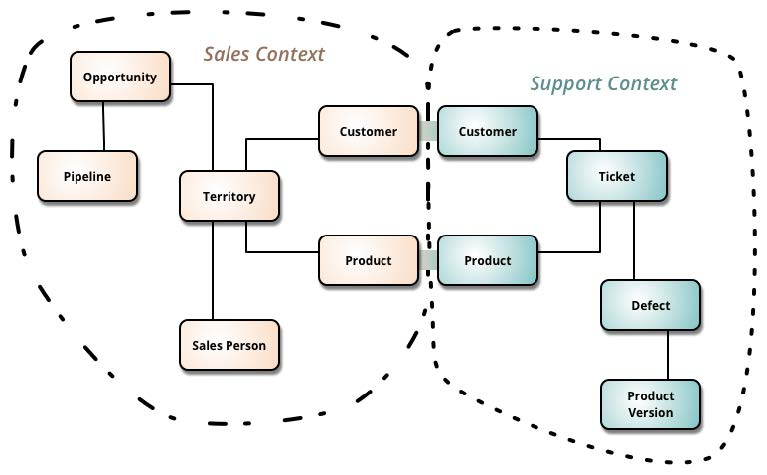
\includegraphics[width=0.9\textwidth]{content/1/chapter1/images/1.jpg}\\
图1.1 - 两个边界上下文,它们之间映射着匹配的术语(图片来自Martin Fowler关于DDD的一篇文章: \url{https://martinfowler.com/bliki/BoundedContext.html})
\end{center}

随着对一些重要的项目管理主题的理解,现在可以转向一些更技术性的主题了。








